
\section{Streaming Readout Upgrade for the sPHENIX trackers}

%As proposed in Chapter~\ref{chap:beam_use_proposal}, 
The nominal sPHENIX data taking assumes calorimeter-based Level-1 triggers for \pp and \pau data taking.  Many sPHENIX observables, such as photons and jets, leave clear signatures in the calorimeter system that can be used to produce such a Level-1 trigger. However, further physics opportunities present only in the non-triggerable data stream. One example is low-\pt open heavy-flavor hadrons that decay hadronically and leave relatively small signals in the
calorimeters when compared with the underlying event. 
These physics channels cannot be efficiently collected via calorimeter triggers, which have too high an energy threshold.
%hadron energy threshold on the order of 10~GeV. 
In the sPHENIX trigger
bandwidth, one would only reasonably allocate 1-5~kHz out of the 15~kHz for the
minimum bias \pp or \pau trigger bandwidth for this type of program. 
% Assuming a
% vertex range selection purity of 50\%, a 1~kHz minimum bias trigger
% leads to recording $2\times10^{-4}$ of the delivered luminosity. 
This translates into rather limited statistics for these rare low-$p_T$ heavy-flavor
signals as quantified in Table~\ref{tab:HFppreach}  (left columns).

The tracking detectors for the sPHENIX experiment all support streaming readout mode, that is where the digitization and readout of the data off the detector does not require Level-1 trigger information as shown in Figure~\ref{fig:TPC-DAQ-structure}. The currently envisioned nominal data taking mode is where the data acquisition selects the time-slice of the tracker data that  corresponds to the calorimeteric-triggered event and saves those time-slices to the output raw data file. 
A streaming readout upgrade in the data acquisition (DAQ) firmware and software is being developed by the collaboration to record a tunable fraction of the tracker data stream on top of the calorimeteric-triggered events, which can vastly increase the fully recorded minimum bias collision event in the full tracking system. 

This hybrid trigger-streaming DAQ is particular efficient in the sense that the recorded events per unit volume of raw data is optimized.  By taking the approach of extending the tracker data recording time window immediately following a calorimeteric-triggered event and completing the partially recorded off-time collisions in the long integration time window of the MVTX and TPC detectors, one captures additional interactions most efficiently. 
From an analysis point of view, this is an elegant solution as it avoids any trigger selection bias which would be quite complicated for rare and weak signals such as hadronically decayed heavy-flavor hadrons.
The working point of this upgrade can be quantified in the data column of the TPC as shown in Figure~\ref{fig:TPC-DAQ-rate}, where a 50\% increase in the data volume column allows for recording 10\% of {\bf all} minimum biased collisions, an increasing by two to three orders of magnitude as detailed in Table~\ref{tab:HFppreach} (right columns). 

% {\textcolor{red}{(Embed something we want PAC to write in report)}} 
% In the first three years of sPHENIX operation, the collaboration
% envisions a run plan sampling 2 trillion \pp collisions (50~\pb) with
% electron and jet triggers, as well as recording 140 billion M.B. \AuAu
% collisions. Comparison of HF observables in heavy-ion collisions to
% those in \pp reveals how the HF probes interact with QGP.  However,
% due to the rareness of the HF signals in the \pp collisions, the
% currently envisioned sPHENIX detector equipped with a traditional
% triggered DAQ cannot efficiently sample HF production below a $p_T$ of
% 10~GeV$/c$.
 

% A detailed study~[{\textcolor{red}{SRO tech note}}] found that the sPHENIX tracking detectors can
% have an upgraded readout mode to record a vast number of \pp collisions via a streaming
% readout upgrade in the data acquisition (DAQ) firmware and software, which is further quantified in  Table~\ref{tab:HFppreach}.
% {\textcolor{red}{(Embed something we want PAC to write in report)}} 


 
% The currently envisioned sPHENIX experiment is designed to take large
% statistics of calorimeter triggered events in the \pp collisions. 
% For observables that utilize the
% calorimeters for analysis, a trigger can usually be designed, such as
% leptonic decays at higher $p_T$, jets, photon, and their correlation
% observables.  
% However, low-$p_T$ ($<10$~GeV$/c$) HF hadrons usually
% decay hadronically and leave relatively small signals in the
% calorimeters when compared with the underlying event. 




\begin{sidewaystable}[thbp]
    \centering
    \begin{tabular}{|c|c|c|c|c|c|} \hline
         & 
         & Year-2, 0-crossing  
         & Year-2, 2mrad-crossing  
         & Year-2, 
         & Year-4  \\ 
         & 
         & in current setup  
         & in current setup  
         & w/ str. tracker
         & w/ str. tracker \\            
         & 
         & Per-1kHz M.B. trigger 
         & per-1kHz M.B. trigger 
         & 
         &  \\ \hline \hline

        M.B.  & Data  
        & Each 1k Hz M.B.  
        & Each 1k Hz M.B.  
        & 10\% M.B. events 
        & 100\% M.B. events \\ 
        p+p & Mode 
        & trigger w/ $2\times10^{-4}$ 
        & trigger w/ $5\times10^{-4}$  
        & str. recorded
        & str. recorded \\ 
         &  
        & of M.B. coll. triggered 
        & of M.B. coll. triggered 
        & 
        & \\ \hline
       
         & Stats 
        & 0.8 Billion M.B. evts 
        & 2 Billion M.B. evts  
        & 400 Billion M.B. evts
        & 5.2 Trillion M.B. evts \\ 
         &  
        & 0.02~\pb recorded 
        & 0.05~\pb recorded 
        & 10.0~\pb recorded
        & 130.0~\pb recorded \\ \hline  
        
        Physics  
        & B $\rightarrow$ D$^{0}$ $\rightarrow$ $\pi$K 
        & 500 evts  
        & 1.2k evts
        & 240k evts 
        & 3M evts \\ 
        Reach &  R$_{AA}$ ref.
        &   
        &  
        & 
        &  \\ \hline          

        & 
        D$^{0} \rightarrow$ $\pi$K pair
        & 500 evts  
        & 1.2k evts
        & 240k evts 
        & 3M evts \\ 
         &  Diffusion of c+$\overline{c}$
        &   
        &  
        & 
        &  \\ \hline 
 
         & 
        $\Lambda_{c} \rightarrow$ $\pi$K$p$ 
        & 1000 evts  
        & 2.5k evts
        & 500k evts 
        & 6.5M evts \\ 
         &  Charm hadronization
        &   
        &  
        & 
        &  \\ \hline 
        
        &
        Prompt D$^{0} \rightarrow$ $\pi$K  
        & 160k evts  
        & 0.4M evts
        & 80M evts 
        & 1B evts \\ 
         & Tri-Gluon Corr. via SSA 
        &   
        &  
        & 
        &  \\ \hline 
        
    \end{tabular}
    \caption{{\textcolor{red}{Number need double check}}Statistical reach for Heavy Flavor \pp measurements by channel in different data taking periods and modes, including streaming readout of the tracker.}
    \label{tab:HFppreach}
\end{sidewaystable}
 




\begin{figure}[htbp]
\begin{center}
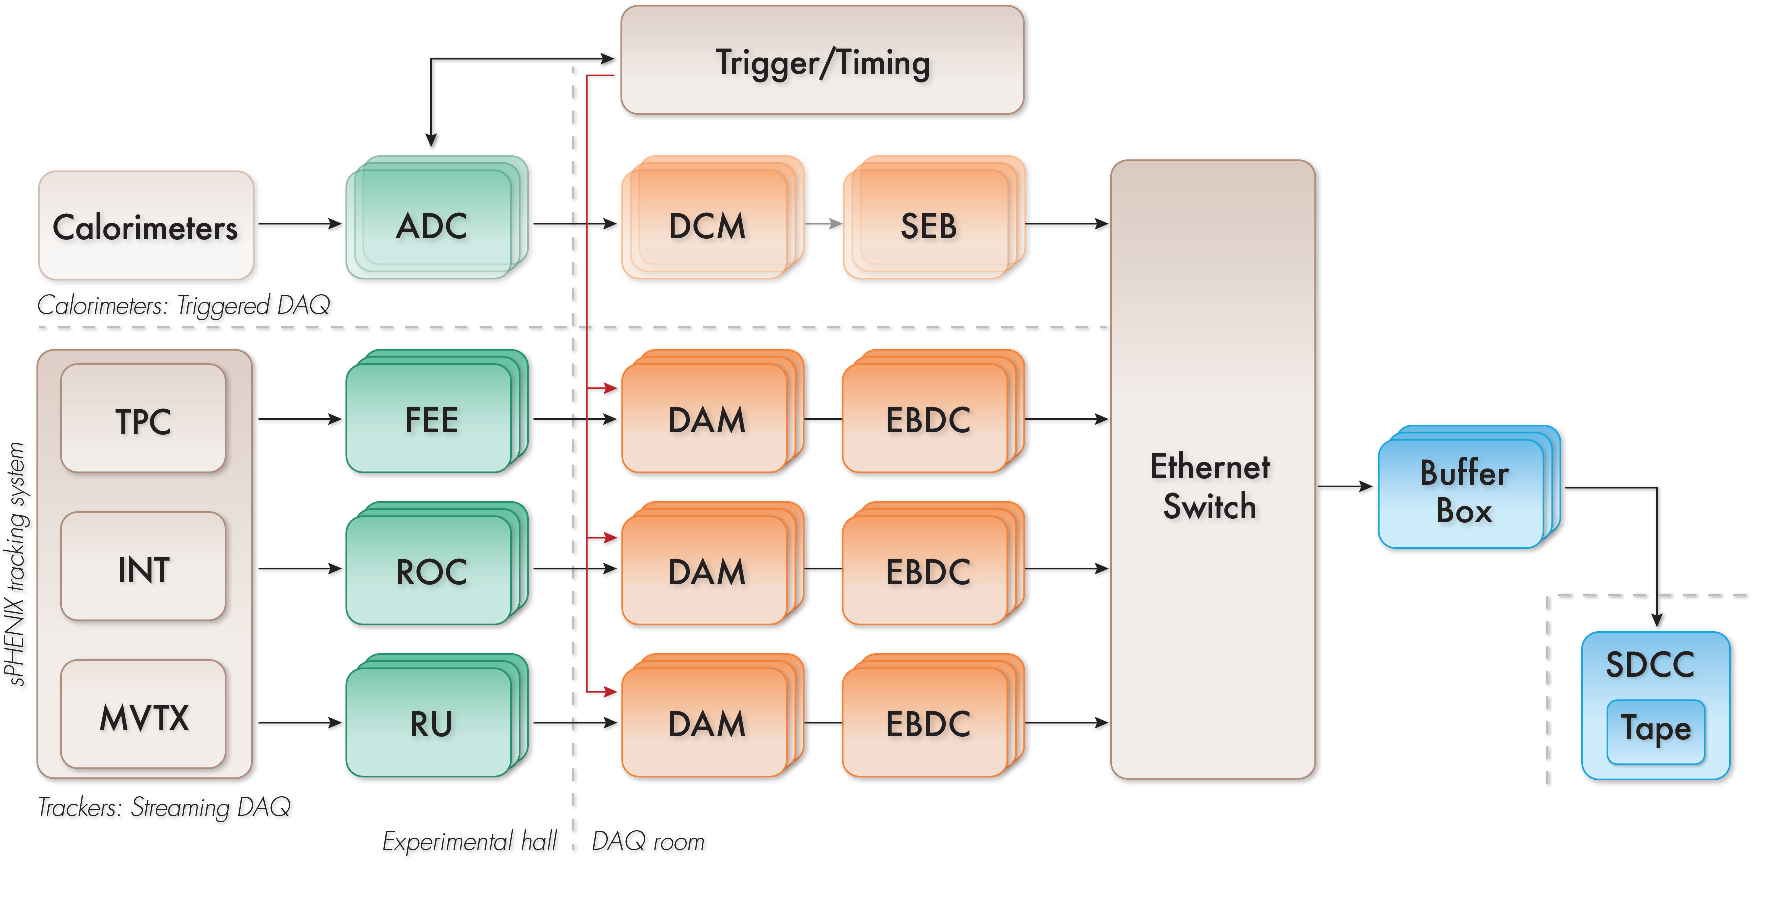
\includegraphics[width=.8\linewidth]{figs/DAQ structure_rev3.pdf}
\caption{The hybrid DAQ structure of the sPHENIX tracking detector, in which  all three tracking detectors are in streaming readout mode. The output of the tracker data stream are throttled to be in synchronize with calorimeter trigger. Additional tracker data can also be streaming to record more minimum bias collisions in addition to the calorimeteric triggered events.}
\label{fig:TPC-DAQ-structure}
\end{center}
\end{figure}
\begin{figure}[htbp]
\begin{center}
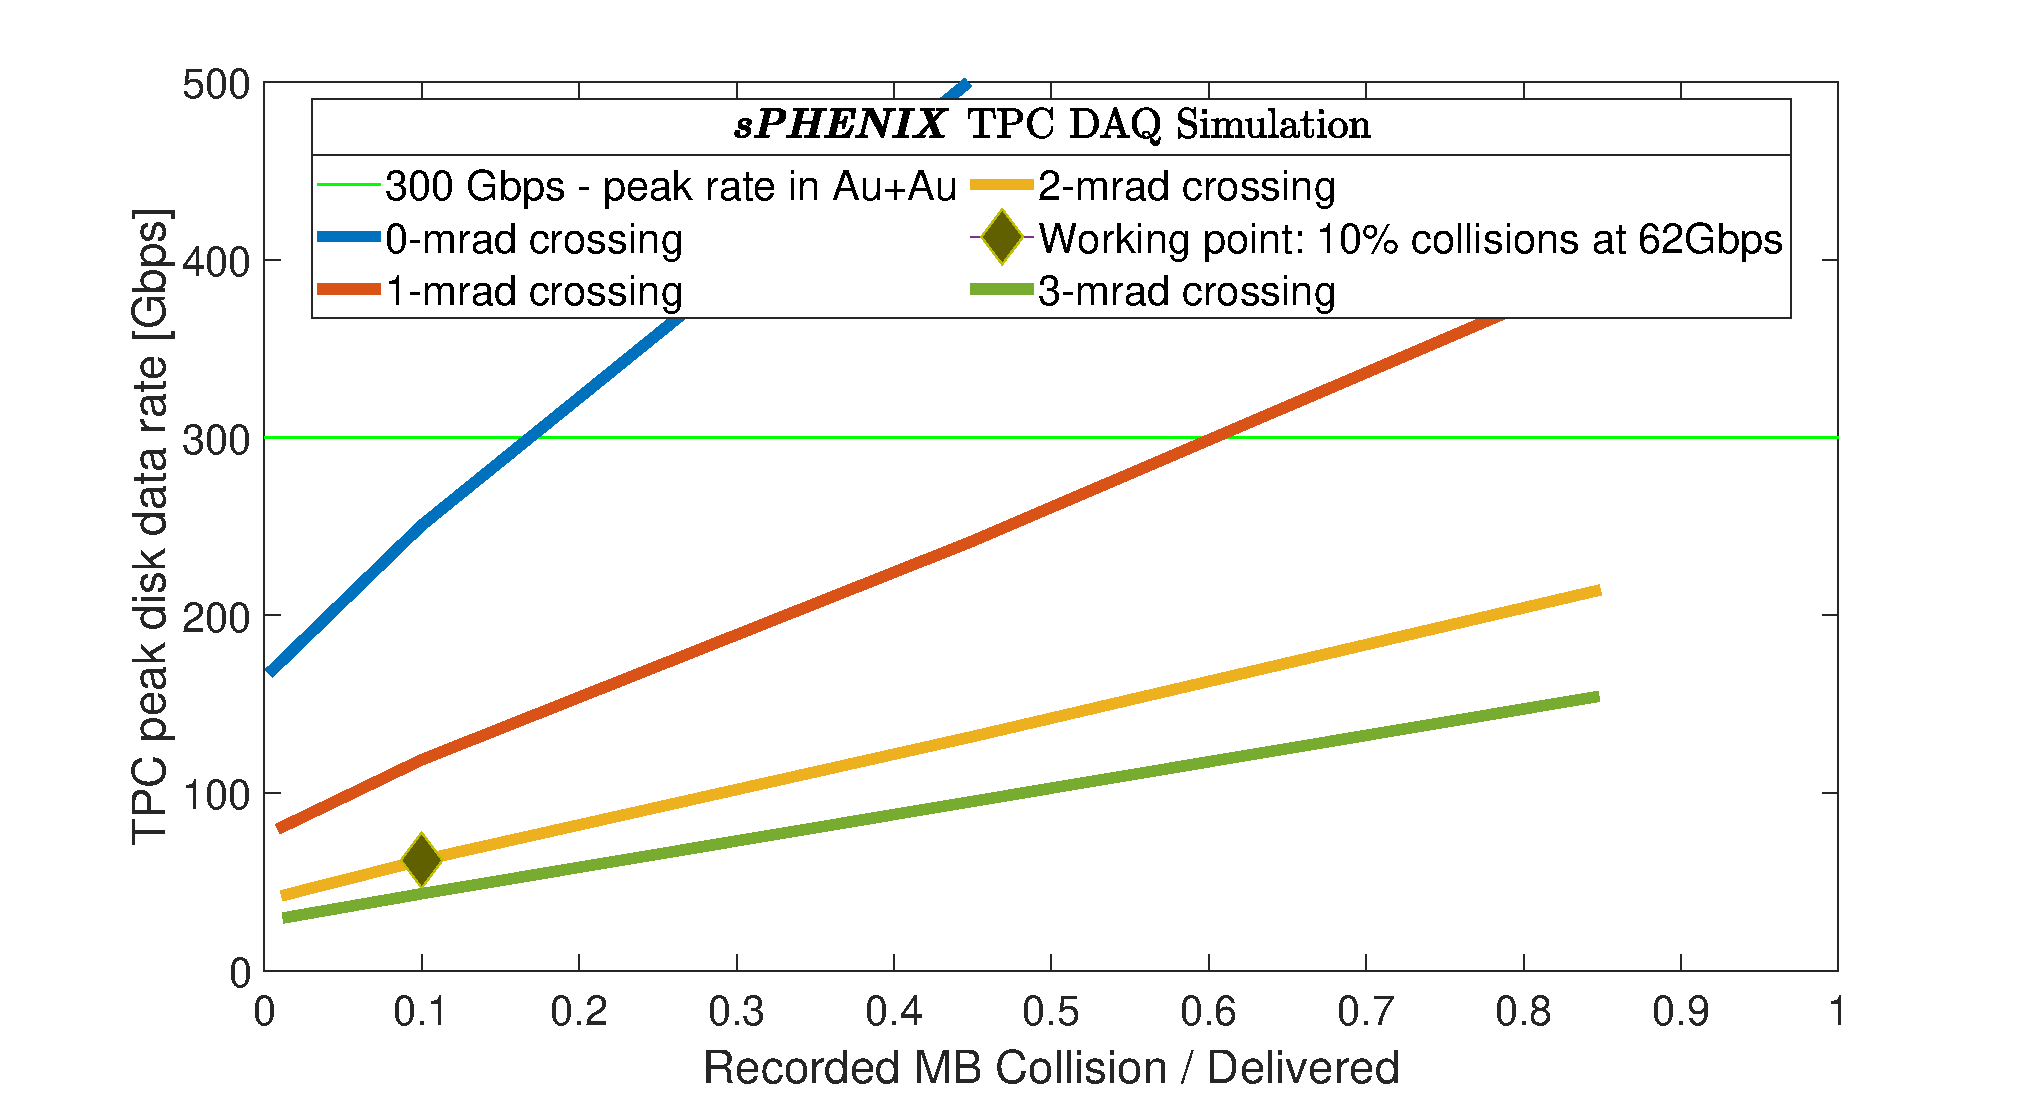
\includegraphics[width=.8\linewidth]{figs/TPCRateLayeredPP_BUP2020_Summary_TriggerWindowRateCoverageCompile.pdf}
% \caption[hoice of operation point between the peak TPC data logging rate and
%   the fraction of M.B. p+p collision recorded.]{\label{fig:TPCRateWindow}
%   Choice of operation point between the peak TPC data logging rate and
%   the fraction of M.B. p+p collision recorded. The green horizontal
%   line denotes the peak data logging rate for Au+Au collisions. At
%   similar logging rate, a minimum of 10\% of \pp M.B. collisions can
%   be streamed to the raw data file as denoted by the solid cyan
%   curve. Other curves denote various online data reduction and beam
%   optimization strategies which would allow recording much higher
%   statistics at a fixed logging rate as further discussed in the last
%   Chapter X.}
\caption{Choice of operation point between the peak TPC data logging rate and the fraction of M.B. p+p collision recorded. The green horizontal line denotes the peak data logging rate for Au+Au collisions. At similar logging rate and without the beam crossing angle, a minimum of 10--20\% of \pp M.B. collisions can be streamed to the raw data file as denoted by the solid blue curve. In the case that a beam cross angle is introduced (red, orange and green curves) the overall data rate can be significantly reduced. The default work point in the 2024 run is with 2~mrad beam crossing angle and record 10\% of collisions at 62 Gbps data rate as denoted by the diamond point.}
\label{fig:TPC-DAQ-rate}
\end{center}
\end{figure}

 
 
\subsection{Hybrid Trigger-Streaming Readout in 2024}
 
In the 2024 run, we plan to implement the first streaming readout DAQ for the tracking detectors to record 10\% of the delivered luminosity in addition to the calorimeteric-triggered events. The data rate and data volume is dominated by the time projection chamber which is studied in Figure~\ref{fig:TPC-DAQ-rate}. With the introduction of the beam crossing angle, the expected data rate with the 10\% streaming readout would be much lower than the design specifications and the previous data volume estimates with zero crossing angle assumed in the 2019 sPHENIX computing plan~\cite{sPH-COMP-2019-001}. The reason is simply because with the 2 milliradian crossing angle there are far fewer collisions outside of $|z|<10$~cm that would have still caused hits in the TPC that would have been recorded.

The physics gain is significant, that includes the \pp reference data for the $D^0$ \raa and the $\Lambda_c/D^0$ ratio both of which are critical for the systematic control in understanding the \AuAu data as discussed in Section~\ref{sec:HF}. In addition, since the \pp beam is transversely polarized, the single spin asymmetry in the $D^0$ channel can be measured to gain access of tri-gluon correlation~\cite{Kang:2008ih, Koike:2011mb}, which is further discussed in Section~\ref{sec:ColdQCD}. 
All aforementioned physics gains would be first measurements at RHIC and uniquely enabled by the streaming DAQ of the sPHENIX trackers.


 
% The upgraded DAQ for the Run2024 \pp and \pA streaming data taking 
% is illustrated in Figure~\ref{fig:TPC-DAQ-structure} and
% summarized in Table~\ref{tab:HFppreach}.  
% The FEE and DAQ hardware of
% each of the three tracking detectors supports a streaming readout mode
% and provides the capability needed for this upgrade. The main work
% will focus on DAQ firmware and software development that enabling the
% streaming capability.  This upgrade would enable the collection of
% sufficient minimum bias in \pp events.  That is, 10\% delivered
% luminosity (see next Chapter) or 200~billion events in the acceptance
% of the vertex tracker, which is a factor of 500 improvement. This
% dataset enables a comprehensive low-$p_T$ hadron program as discussed
% here.  The analysis of these HF hadronic channels does not require
% calorimeter information. Instead, they can be identified with the precision
% tracking detectors of sPHENIX (at $p_T=5$~GeV$/c$, $\sigma(p)/p=1\%$,
% $\sigma(DCA)<10$~$\mu$m ) via a combination of decay topology and
% invariant mass, as demonstrated for even the busiest events of Au+Au
% collisions through detailed simulation studies in~\cite{sPH-HF-2017-002}.

% As summarized in Table~\ref{tab:HFppreach}, an upgraded DAQ for
% sPHENIX trackers will enable the recording of 500 times greater
% statistics of M.B. \pp collisions, which in turn will enable proper HF
% measurements in this key kinematic region.


\subsection{Full streaming Readout for Potential 2026-2027 Running}

In the potential running in 2026 to 2027, we plan to build on the initial experience with streaming readout and aim for stream recording 100\% data stream for the sPHENIX tracking detectors for all collision species. As shown in Figure~\ref{fig:TPC-DAQ-rate}, the data rate would be significantly higher compared the the 2024 work point, but would still be below the bandwidth limit of the readout system. At the expense of higher data volume, full streaming readout of the tracker allows another order of magnitude improvement in the recorded \pp and \pA collision, whose impact is further quantified in Chapter~\ref{chap:beam_use_proposal_extra}.

\subsection{Data Preservation and Data Mining}

This upgrade will accumulate a large amount (10-100\% of delivered luminosity) 
of minimum
bias polarized \pp collision without a trigger bias and with the full
sPHENIX tracking capability and preserved at RHIC computing facility. 
After RHIC completes its scientific
mission at the end of the sPHENIX program, this unique dataset would  allow future data mining for novel quantum effects such as
the quantum coherence in particle productions. 
Such future analysis would have full freedom to define an ``event'' in the offline software ``trigger'' that is based on high level objects such as tracklets and final detector alignment and calibrations. 
These \pp data may be
critical for understanding the future $e+p/A$ collision data at an
Electron Ion Collider~\cite{Accardi2012}.
